\documentclass[10pt,letterpaper]{article}

% -----------------------------------------------------------------------------
% SCA 2.0 position paper v3 — self-contained pdflatex source
% -----------------------------------------------------------------------------
\usepackage[margin=0.88in,top=0.82in,bottom=0.82in]{geometry}
\usepackage{mathptmx}
\usepackage[T1]{fontenc}
\usepackage{microtype}
\usepackage{amsmath,amssymb}
\usepackage{amsthm}
\newtheorem{proposition}{Proposition}[section]
\newtheorem{definition}{Definition}[section]
\newtheorem{remark}{Remark}[section]
\newtheorem{assumption}{Assumption}[section]
\usepackage{booktabs,array,tabularx}
\usepackage{graphicx}
\usepackage{tikz}
\usetikzlibrary{arrows.meta,positioning,shapes.geometric,calc}
\usepackage{xcolor}
\usepackage{hyperref}
\usepackage{enumitem}
\usepackage{titlesec}
\usepackage{caption}
\usepackage{fancyhdr}
\usepackage{multicol}

\definecolor{econblue}{RGB}{20,55,95}
\definecolor{slate}{RGB}{79,89,104}
\definecolor{mist}{RGB}{242,245,249}
\definecolor{rulegray}{RGB}{203,210,220}
\definecolor{warm}{RGB}{132,85,38}
\definecolor{green}{RGB}{42,104,78}

\hypersetup{colorlinks=true,linkcolor=econblue,citecolor=econblue,urlcolor=econblue,
  pdftitle={Synthetic Cultural Agents 2.0: Adjudicating Cheap Measurements},
  pdfauthor={Augusto Gonzalez-Bonorino, Kseniia Biriukova, and Monica Capra}}
\setlength{\parindent}{1.15em}
\setlength{\parskip}{0.18em}
\setlength{\headheight}{15pt}
\titlespacing*{\section}{0pt}{1.0em}{0.3em}
\titlespacing*{\subsection}{0pt}{0.68em}{0.22em}
\titleformat{\section}{\large\bfseries\color{econblue}}{\thesection.}{0.55em}{}
\titleformat{\subsection}{\normalsize\bfseries\color{econblue}}{\thesubsection}{0.45em}{}
\setlist[itemize]{leftmargin=1.3em,itemsep=0.12em,topsep=0.15em}
\setlist[enumerate]{leftmargin=1.45em,itemsep=0.12em,topsep=0.15em}
\captionsetup{font=small,labelfont={bf,color=econblue},skip=4pt}

\pagestyle{fancy}
\fancyhf{}
\fancyhead[L]{\small\color{slate} EconLLM Lab \textperiodcentered\ SCA 2.0 position paper}
\fancyhead[R]{\small\color{slate}\thepage}
\renewcommand{\headrulewidth}{0.35pt}
\renewcommand{\headrule}{\hbox to\headwidth{\color{rulegray}\leaders\hrule height \headrulewidth\hfill}}
\fancypagestyle{plain}{\fancyhf{}\fancyfoot[C]{\small\color{slate}\thepage}\renewcommand{\headrulewidth}{0pt}}

\newcommand{\SCA}{\textsc{sca}}
\newcommand{\LLM}{\textsc{llm}}
\newcommand{\DPO}{\textsc{dpo}}
\newcommand{\GPS}{\textsc{gps}}
\newcommand{\WVS}{\textsc{wvs}}
\newcommand{\WEIRD}{\textsc{weird}}
\newcommand{\cvp}{\texttt{cvprofiles}}
\newcommand{\M}{\ensuremath{\mathcal{M}}}
\newcommand{\E}{\mathbb{E}}

\begin{document}

% -----------------------------------------------------------------------------
% Cover (excluded from the paper-length target)
% -----------------------------------------------------------------------------
\thispagestyle{empty}
\begin{center}
\vspace*{1.3cm}
{\color{econblue}\rule{\textwidth}{1.15pt}}\\[0.45em]
{\LARGE\bfseries\color{econblue} Synthetic Cultural Agents 2.0:}\\[0.16em]
{\LARGE\bfseries\color{econblue} Adjudicating Cheap Measurements}\\[0.45em]
{\color{econblue}\rule{\textwidth}{0.55pt}}\\[0.85em]
{\large A position paper on validated AI measurement for non-\WEIRD{} populations}\\[1.0em]
{\large\textbf{Augusto Gonzalez-Bonorino}\textsuperscript{1}\quad
\textbf{Kseniia Biriukova}\textsuperscript{2}\quad
\textbf{Monica Capra}\textsuperscript{1,3}}\\[0.5em]
{\small\textsuperscript{1}Department of Economics, Arizona State University; EconLLM Lab.\\
\textsuperscript{2}EconLLM Lab.\\
\textsuperscript{3}Department of Economics, Claremont Graduate University; EconLLM Lab.}\\[0.8em]
{\normalsize August 2026 \textperiodcentered\ Working paper / position paper}\\[0.4em]
{\color{econblue}\rule{0.28\textwidth}{0.35pt}}
\end{center}

\vfill
\noindent\colorbox{mist}{\parbox{0.965\textwidth}{\small\vspace{0.25em}
\textbf{Status.} This paper sets a research standard rather than claiming that the standard has already been met. The current SCA 2.0 adapter evidence is a two-country proof of concept. It supports neither calibrated population prediction nor a general superiority claim over persona prompting. The proposed validation program is the condition for those claims. Code is available at \href{https://github.com/EconLLM-Lab/SCA2_PofW}{\texttt{github.com/EconLLM-Lab/SCA2\_PofW}}; the companion validation engine is \href{https://github.com/Bonorinoa/cvprofiles}{\texttt{cvprofiles}}.\vspace{0.25em}}}
\newpage

\section*{Statement of significance}
Generative models have made candidate measurements of latent constructs --- trust, religiosity, cultural preferences --- cheap to produce. Any prompt, fine-tuning procedure, or survey composite now yields a measurement function at near-zero marginal cost, and validity, not supply, has become the bottleneck of empirical work that relies on such measurements. This paper treats every artificial-intelligence procedure as a candidate measurement of a latent construct and screens it against theory-derived restrictions and independent human data, then reports which downstream conclusions survive the screen. The protocol is implemented in an open, auditable software tool that any researcher can apply to any construct and any candidate measurement. The payoff is disciplined hypothesis generation and measurement selection --- an adjudication procedure for a crowded marketplace of measurements --- not a synthetic substitute for fieldwork.

\section*{Abstract}
Artificial intelligence has made candidate measurements of latent constructs nearly free: any persona prompt, preference-trained model, or survey composite yields an operationalization of a construct such as trust or cultural preference on demand. Validity is now the scarce resource. \emph{Ex ante}, no operationalization is privileged, and synthetic survey responses are known to diverge from real data in a large share of estimable quantities. This paper provides an end-to-end framework for adjudicating among candidate measurements. It turns a researcher's theoretical commitments into testable moment-inequality restrictions; screens candidate measurement functions against those restrictions and against independent human data; characterizes the admissible set of measurements that survive; and reports the range of downstream conclusions consistent with that set, with inference that remains valid despite the data-dependent screening step. The framework is implemented in an open-source, model-free software package built for auditability, and it completes the estimation and inference layer of a construct-validity program that recent NBER Methods work called for but explicitly deferred. The application measures latent cultural preferences in non-\WEIRD{} populations, with trust as a flagship construct, and trains synthetic cultural agents from population-level survey moments. The falsifiable core of the program is that measurement selection guided by construct validity predicts validity evidence it was not optimized to satisfy, assessed on pre-registered held-out restrictions. The present results are a proof of concept; the contribution is the standard and the framework.

\noindent\textit{Keywords:} AI measurement; synthetic populations; cultural preferences; construct validity; partial identification; Direct Preference Optimization; non-\WEIRD{} populations

\section{The problem: cheap simulations, weak warrants}
Social scientists have long measured latent attributes such as trust, patience, reciprocity, and risk tolerance with surveys, experiments, and behavioral traces. None of these instruments is the attribute itself. Each is a representation whose usefulness depends on what it preserves and what it distorts. Large language models make one more representation extraordinarily cheap: a researcher can ask a model to answer as a member of a target population and obtain a synthetic sample in minutes \cite{horton2023,argyle2023,aher2023}. The practice has spread quickly from single-shot simulated respondents to annotation pipelines and persistent agent populations \cite{ziems2024,park2024}.

This convenience changes the bottleneck. The hard question is no longer whether a researcher can generate an answer; it is whether the procedure that generated it measures anything stable about the intended population. This question is especially sharp outside the populations most visible in the data, annotator pools, and institutional settings that shape leading models. The concern is not that an AI system is ``biased'' in the abstract. It is that an unvalidated projection from a target population to an AI response can silently inherit a \WEIRD{} default, a prompt artifact, or a model-specific prior \cite{henrich2010,durmus2024}.

\SCA{} 1.0 showed that carefully constructed persona prompts can reproduce non-\WEIRD{} patterns in economic experiments \cite{capra2025}. That result establishes persona prompting as a serious benchmark, not a straw man. But it remains an inference-time procedure: the cultural signal is supplied in a transient context, the features of that context that carry the signal are hard to isolate, and a model update can change the result without changing the social-science theory.

\begin{figure}[t]
\centering
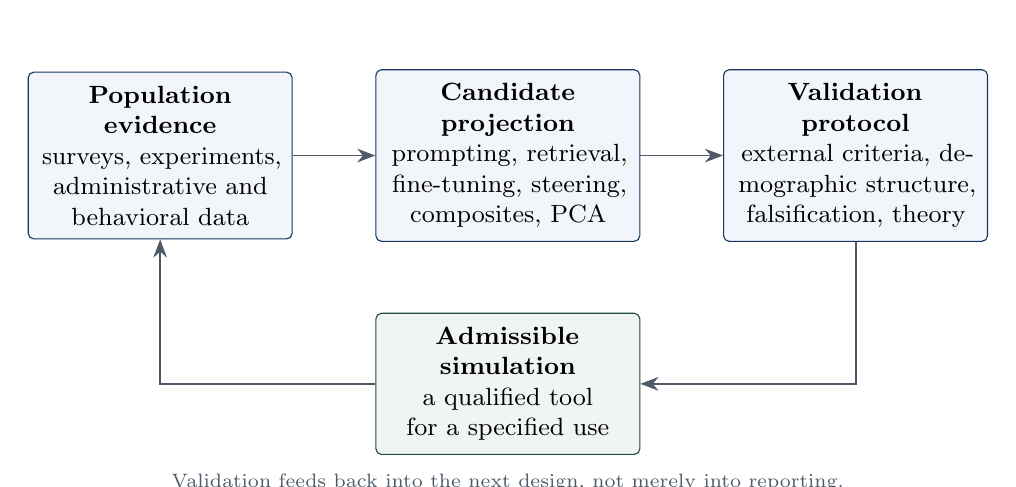
\begin{tikzpicture}[font=\small,
 box/.style={draw=econblue, rounded corners=2pt, fill=mist, align=center, text width=3.0cm, minimum height=1.0cm, inner sep=5pt},
 validbox/.style={draw=green!75!black, rounded corners=2pt, fill=green!7, align=center, text width=3.0cm, minimum height=1.0cm, inner sep=5pt},
 arr/.style={-{Stealth[length=2.3mm]}, line width=.7pt, color=slate}]
\node[box] (evidence) {\textbf{Population evidence}\\surveys, experiments, administrative and behavioral data};
\node[box, right=1.05cm of evidence] (function) {\textbf{Candidate projection}\\prompting, retrieval, fine-tuning, steering, composites, PCA};
\node[box, right=1.05cm of function] (test) {\textbf{Validation protocol}\\external criteria, demographic structure, falsification, theory};
\node[validbox, below=0.9cm of function] (output) {\textbf{Admissible simulation}\\a qualified tool for a specified use};
\draw[arr] (evidence)--(function);
\draw[arr] (function)--(test);
\draw[arr] (test.south) |- (output.east);
\draw[arr] (output.west) -| (evidence.south);
\node[font=\scriptsize\color{slate},below=.12cm of output] {Validation feeds back into the next design, not merely into reporting.};
\end{tikzpicture}
\caption{The proposed research loop. A simulation is not validated by sounding plausible or by agreeing with another AI system. It earns a limited use claim only after a prespecified projection function survives external and theoretical tests.}
\label{fig:loop}
\end{figure}

The empirical record now justifies treating this worry as the field's central problem rather than a footnote. Synthetic survey replacements match ANES averages but differ significantly from the ANES benchmark on 48\% of estimated coefficients, with sign flips in 32\% of those cases \cite{bisbee2024}. A 2026 study built on \WVS{} data and more than 70{,}000 respondent--item observations finds that multi-attribute persona prompting yields no clear aggregate improvement and can worsen subgroup fidelity \cite{morocho2026}. GPT-4.1 reaches only 57.4\% modal-preference accuracy on subgroup cultural values, and fine-tuning---not prompting---substantially improves out-of-domain subgroup prediction \cite{subgroupvalues2026}; demographic cues prove unstable across 14.8 million prompts \cite{tonneau2026}; culture-conditioned prompting improves alignment with survey responses for most countries, but not all \cite{tao2024}; and calibration emerges as a validity component in its own right across fourteen constructs \cite{wangcalibration2026}. Yet the measurement turn is equally real: at the 2026 PolMeth meeting, 45 of 175 presentations (26\%) centrally involve generative AI, and 60\% of those concern measurement---annotation and measurement beyond labeling \cite{hall2026}. LLMs annotate text at least as accurately as crowd workers \cite{gilardi2023}, although reliable coding of open-ended responses requires fine-tuning rather than prompting \cite{landesvatter2026}. The field is therefore in an uncomfortable position: the measures are multiplying faster than the warrants.

Economics never imported the psychometric apparatus wholesale because it had substitutes. The measurement-error tradition---attenuation, instrumental variables, nonclassical measurement error---absorbed the inference agenda: when a variable is mismeasured, one corrects; one does not validate \cite{hu2008,chen2011,schennach2021}. The trust literature, meanwhile, has been doing implicit convergent, discriminant, and criterion validation for a quarter century without the vocabulary: survey trust against experimental behavior \cite{glaeser2000}, the attitude--trust distinction against revealed trustworthiness \cite{sapienza2013}, trust against real economic outcomes \cite{butler2016}, and the Global Preferences Survey (\GPS{}) validated ex ante against incentivized experiments, test--retest reliability, and cross-country invariance \cite{falk2018,falk2023}. What was missing was not the questions but the menu. With a single affordable proxy, validation means defending that proxy; menu and adjudication problems are invisible until AI makes candidate measures cheap. Now they are cheap, and the menu problem is everyone's.

The conceptual machinery for answering it now exists. Dell and Rambachan's NBER 2026 program formalizes the Cronbach--Meehl nomological network \cite{cronbach1955} as partial identification: a menu of measurement functions generates moment-inequality restrictions, an admissible set of measures, and a construct-identified interval $[L,U]$ for downstream conclusions \cite{dellrambachan2026}. Their Methods Lecture defers estimation as beyond its scope, and the companion article treats \LLM{}s as an applied econometric framework \cite{ludwig2026}. We complete this program end-to-end: the inference layer, the open implementation \cvp{} \cite{cvprofiles}, and culture as the first application. Section~3 formalizes the framework; the remainder of the paper applies it.

\SCA{} 2.0 asks whether cultural variation can instead be represented in an estimable policy and subjected to the same external discipline expected of any measurement instrument. The paper's question is two-part. First, can a policy trained on culture-labeled preference data---rather than a prompt---reproduce externally observed human outcomes on preregistered tests, and does it improve on persona prompting under the same conditions? Second, does the resulting measure survive construct validation: is its admissible set nonempty, and is the construct-identified interval $[L,U]$ informative? The existing two-country adapter evidence motivates these questions but is a proof of concept, not an answer \cite{capra2025}.

The next section reviews the converging literatures in which this program sits.
\clearpage

\section{Related literature}

The measurement problem sits at the intersection of four literatures that have developed largely in parallel.

\subsection{Synthetic subjects: from personas to policies}

The use of large language models as simulated respondents began with demonstrations of feasibility. Horton, Filippas, and Manning~\cite{horton2023} introduced ``Homo Silicus,'' using \LLM{}s as stand-in economic agents in laboratory-style experiments; Argyle et al.~\cite{argyle2023} showed that demographically conditioned models can approximate the response distributions of matched human survey samples, a procedure they called silicon sampling; and Aher et al.~\cite{aher2023} proposed the Turing experiment as a general template for eliciting beliefs from models. Manning, Zhu, and Horton~\cite{manning2024} pushed the program toward automated social science, treating structural causal models as explicit blueprints whose simulated populations are populated by \LLM{} agents---an end-to-end framework for \emph{constructing} simulated subjects, distinct in purpose from the end-to-end framework for \emph{adjudicating} measurements developed here---while Park et al.~\cite{park2024} demonstrated the behavioral plausibility of generative-agent populations in a sandbox environment. The survey-simulation literature matured in parallel, cataloguing the design space of \LLM{} respondents~\cite{ziems2024}.

That enthusiasm met a wave of quantitative skepticism. Bisbee et al.~\cite{bisbee2024} found that 48\% of coefficients estimated from \LLM{} survey responses differed from those obtained from human samples; a large-scale replication across more than 70{,}000 World Values Survey respondents reached similarly sobering conclusions about naive prompting~\cite{morocho2026}. Accuracy degrades unevenly across subgroups---GPT-4.1 attained 57.4\% subgroup-level accuracy in a cross-national values benchmark, with fine-tuning the most reliable remedy~\cite{subgroupvalues2026}---and the demographic cues used for conditioning are themselves unstable~\cite{tonneau2026}. Cultural prompting does not transfer across contexts~\cite{tao2024}, stated preferences are systematically miscalibrated~\cite{wangcalibration2026}, and off-the-shelf models require fine-tuning before their text coding is usable~\cite{landesvatter2026}.

The field's response has been to move from prompts to trained policies. PLURAL built preference models on roughly 500{,}000 preference triplets drawn from the Integrated Values Survey across 20 countries~\cite{plural2026}; PALMs trained population-aligned per-country models and report that construct-grounded rationales outperform both demographic prompting and survey-based fine-tuning~\cite{palms2026}. Training is not the only route: DISCA instantiates each country as a panel of World Values Survey-grounded persona agents and applies an inference-time logit correction, reducing cultural misalignment without changing weights~\cite{disca2026}. That claim---that training on survey responses is the benchmark to beat---defines the standard of comparison the closing paragraph addresses.

\subsection{The measurement turn}

In parallel, \LLM{}s have become measurement infrastructure in the social sciences. Gilardi et al.~\cite{gilardi2023} showed that models annotate text at scale with accuracy rivaling crowd workers; Ziems et al.~\cite{ziems2024} and Landesvatter et al.~\cite{landesvatter2026} extended the case to text scaling and coding, and Halterman and Keith proposed a five-stage framework for evaluating codebook \LLM{}s as measurement instruments for political-science concepts~\cite{halterman2024}. The 2026 Political Methodology conference census documents the trajectory: 45 of 175 core presentations involved AI, and roughly 60\% of those were measurement-related~\cite{hall2026}. The measurement framing has reached methodology proper: Licht~\cite{licht2025} compared four protocols for eliciting scalar constructs---pointwise prompting, pairwise comparisons, token-probability scoring, and fine-tuning---treating the choice among them as a measurement decision, calibration has been treated as a validity component across fourteen constructs~\cite{wangcalibration2026}, and a systematic audit of validation practice across eight flagship social-science journals finds \LLM{}-based measurement inconsistent and limited~\cite{desai2026}. The same turn is visible in machine-learning benchmarking: a systematic review of 445 \LLM{} benchmarks calls for construct validation~\cite{bean2025}, benchmarks have been argued to require nomological networks~\cite{freiesleben2026}, and discriminant validity of predictive algorithms can be falsified directly~\cite{coston2026}. What these literatures share is the recognition that measurement, not prediction, is the central epistemic act, and that validity is the property to be audited.

\subsection{Construct validity in economics: the absent apparatus}

The apparatus for that audit exists, but outside economics. Cronbach and Meehl~\cite{cronbach1955} defined construct validity as the placement of a measure within a nomological network of theoretical relations; Campbell and Fiske~\cite{campbell1959} supplied the multitrait-multimethod matrix for detecting method variance; Borsboom et al.~\cite{borsboom2004} argued that a network of associations is not a causal account of measurement; and Messick~\cite{messick1995} and Kane~\cite{kane2013} broadened validity into an argument-based enterprise spanning evidence and consequences. Economics never imported this apparatus. The measurement-error tradition absorbed its inference agenda---attenuation, instrumental variables, nonclassical measurement error, and repeated measures~\cite{hu2008,chen2011,schennach2021}---while the trust literature performed convergent, discriminant, and criterion validation for a quarter century without the vocabulary: Glaeser et al.~\cite{glaeser2000} questioned the behavioral content of the survey item, Sapienza et al.~\cite{sapienza2013} decomposed the World Values Survey trust item into beliefs and preferences, Butler et al.~\cite{butler2016} validated trust measures against behavior, and the Global Preferences Survey was validated ex ante against incentivized experiments and across countries~\cite{falk2018,falk2023}. The trigger for importing the apparatus is cost: when AI makes a menu of candidate measures cheap to produce, validation ceases to be the defense of a single proxy and becomes the adjudication of a menu---a problem that requires a formal selection device.

\subsection{The bridge and the frontier}

That device is arriving from econometrics. Dell and Rambachan's 2026 NBER Methods Lecture formalizes the nomological network as a partial-identification problem: a menu of candidate measures, moment-inequality restrictions derived from theory, an admissible set, and a resulting construct-identified interval, with inference explicitly deferred~\cite{dellrambachan2026}; Ludwig develops the companion econometric framework for \LLM{} measurement~\cite{ludwig2026}. Ogut and Yin~\cite{ogutyin2026} derive loading-invariant intervals for a latent regressor from curvature bounds with multiple nonlinear measurements, and Chen, Rambachan, and Tamer~\cite{chenrambachantamer2026} derive partial-identification bounds for latent prevalence from panels of LLM reports, disciplining the mixture with externally calibrated scores in the spirit of the misclassification literature. These build on the classical partial-identification toolkit~\cite{manski2003} and the theory of measurement systems~\cite{schennach2021}, and Molinari~\cite{molinari2020} has raised directly the question of what econometrics should import from psychometrics.

\paragraph{The gap.}
Each ingredient now exists separately: elicitation menus \M{}~\cite{licht2025}; admissible sets from moment restrictions, presented as an argument with inference deferred~\cite{dellrambachan2026}; identified intervals over measures via curvature bounds, without a theory-restricted menu or a psychometric bridge~\cite{ogutyin2026}; survey-anchored preference training~\cite{plural2026,palms2026}; and a per-measure Construct Validity Protocol for embedding-based social measures~\cite{proxy2026}. The last validates individual operationalizations against discriminant, incremental, and predictive tests; the framework below takes the menu, not the measure, as the object of inference. No existing treatment, however, (i) uses theory-restricted admissible sets as the selection device that narrows \M{} to defensible measures; (ii) propagates the coupled uncertainty of admissibility and target parameter into valid inference; (iii) implements the entire protocol in an auditable open tool; or (iv) applies it to AI-generated cultural measurement. This paper supplies that treatment: \cvp{} operationalizes construct validity as partial identification over \M{}, and the moment-anchored estimator proposed here is not response-surface fine-tuning---it is a discrete-choice policy identified from population-level moments, which is exactly the object a validity framework can screen. The screening question, not the raw policy, is the point of the paper.

\section{A general framework for validated AI measurement}
\subsection{Projection functions, not one privileged method}
Let $X$ denote evidence about a target population and let $Y$ be an outcome relevant to a scientific question. A procedure $m_j$ maps available inputs into a score, choice distribution, or simulated response: $m_j(X)$. We call $m_j$ a \emph{projection function}. The term is deliberately broader than ``model.'' It includes a survey composite, a principal component, an experimental outcome, and an AI-based procedure.

The distinction among AI procedures still matters. Persona prompting and retrieval-augmented generation are \emph{contextual projections}: they leave the policy fixed and change the information supplied at inference. Fine-tuning and activation steering are \emph{policy interventions}: they change the policy whose responses are later scored. In all four cases, the object that enters an empirical analysis is the evaluated output $m_j(X)$, so each belongs in the same measurement menu. Calling them all ``measurement'' is accurate only in this downstream sense; it should not obscure their different causal and engineering properties.

For SCA 2.0, the menu should be explicit before results are inspected:
\[
\M=\{m_{\mathrm{persona}},m_{\mathrm{RAG}},m_{\mathrm{base}},m_{\mathrm{DPO}},m_{\mathrm{steer}},m_{\mathrm{composite}},m_{\mathrm{PCA}},m_{\mathrm{experiment}}\}.
\]
The last three entries are crucial. A DPO agent should not be compared only with other LLMs. Survey composites and PCA are transparent statistical alternatives; incentivized experimental measures and held-out human survey outcomes provide different-method criteria. Agreement among several prompted models is not construct validity because their errors may be correlated \cite{campbell1959,ludwig2026}.

\subsection{Validation as partial identification}
Construct validity asks whether a score can support a stated interpretation. Cronbach and Meehl's answer was a \emph{nomological network}: a valid measure should bear theoretically specified relations to other observables \cite{cronbach1955}. The framework below converts that idea into an auditable decision rule.

A researcher defines a construct $C$, a finite menu $\M$, auxiliary observables $V$, and restrictions $r\in\mathcal{R}$. Each restriction has a literature-anchored threshold $\theta_r$:
\begin{equation}
 r:\qquad \E\left[g_r\{m_j(X),V;\theta_r\}\right]\geq 0.
 \label{eq:restriction}
\end{equation}
The sample analogue $s_r(m_j)$ is the restriction's slack. With tolerance $\delta\geq0$, the admissible measures are
\begin{equation}
 \M^*=\left\{m_j\in\M:s_r(m_j)\geq-\delta\quad \forall r\in\mathcal{R}\right\}.
 \label{eq:admissible}
\end{equation}
For a downstream target $\beta(m)$, such as a treatment-effect estimate or correlation with an economic outcome, the honest estimand is not automatically a single number. It is the construct-identified set
\begin{equation}
 \mathcal{B}^*=\{\beta(m):m\in\M^*\},\qquad [L,U]=[\min\mathcal{B}^*,\max\mathcal{B}^*].
 \label{eq:range}
\end{equation}
This is partial identification: data and stated assumptions determine a set of conclusions, not more \cite{manski2003,schennach2021}. \cvp{} implements this sequence---score, restrict, identify, report---with frozen inputs, a full slack profile, bootstrap uncertainty over units, and threshold-sensitivity diagnostics. It does not choose the construct or write the network. Those remain the researcher's responsibility.

Passing these restrictions means that a measure is consistent with the nominated network. It does not prove that the latent attribute causes the score, that the construct is uniquely defined, or that the policy can answer arbitrary questions about a population \cite{borsboom2004}. Empty admissible sets and wide ranges are useful outcomes: they tell the researcher that the current evidence does not warrant the intended interpretation.

\paragraph{Maintained assumptions.}
Every application of the framework rests on four assumptions. They are stated once and used everywhere; they are the researcher's commitments, not outputs of the engine. Conversely, any implication of the framework that could be wrong is treated as testable: whenever a derived consequence can be checked against data, it should be promoted to a restriction in $\mathcal{R}$, and it is the audit role of \cvp{} to run that check. Maintained assumptions are thereby kept minimal and visible, while testable content migrates into the network, where it can falsify measures.

\begin{enumerate}
\item[(A1)] \emph{Menu coverage.} The menu $\M$ contains the operationalizations of interest for the research question: persona prompts, fine-tuned policies, survey composites, factor scores, experimental outcomes, or any other candidate measurement function the researcher is willing to defend. Coverage is argued from the literature and the research design; it is never proven, and the menu remains researcher-supplied throughout.
\item[(A2)] \emph{Restriction validity.} Each restriction $g_r\in\mathcal{R}$ is a correct testable implication of the construct definition together with the auxiliary evidence $V$: the population moment $\E[g_r(m(X),V;\theta_r)]\ge 0$ holds for every admissible $m$. The restrictions are researcher-owned---they encode the nomological network the researcher asserts---and each is falsifiable by the data, in the sense that violation is an observable event.
\item[(A3)] \emph{Sampling.} The unit-by-measure score matrix from which $\hat{s}_r(m)$ and $\hat{\beta}(m)$ are computed is drawn under a stated sampling model. For the cultural application the model is exchangeability of country-level aggregates: the $n$ country observations are exchangeable draws from the target population of countries, so that resampling units approximates the sampling distribution. The model is stated per application and frozen with the run.
\item[(A4)] \emph{Tolerance policy.} The tolerance $\delta\ge 0$ is declared ex ante and defaults to zero; it is never tuned to rescue an empty admissible set. A positive $\delta$ is a substantive statement about how literally the researcher holds the network---slack is admitted into the restrictions---and every reported object is $\delta$-conditional.
\end{enumerate}

\paragraph{Consistency.}
The sample objects are the plug-in admissible set $\hat{\M}^*=\{m\in\M:\hat{s}_r(m)\ge-\delta\ \forall r\}$ and the plug-in range $[\hat L,\hat U]$, with $\hat L=\min_{m\in\hat{\M}^*}\hat{\beta}(m)$ and $\hat U=\max_{m\in\hat{\M}^*}\hat{\beta}(m)$. Proposition~\ref{prop:consistency} gives the minimal conditions under which these converge to their population counterparts.

\begin{proposition}[Consistency of the admissible set and the construct-identified range]\label{prop:consistency}
Assume A1--A4. Suppose the slack estimators are uniformly consistent for their population analogues,
\begin{equation}
\max_{m\in\M}\max_{r\in\mathcal{R}}\bigl|\hat{s}_r(m)-s_r(m)\bigr|\xrightarrow{p}0,
\qquad
\max_{m\in\M}\bigl|\hat{\beta}(m)-\beta(m)\bigr|\xrightarrow{p}0,
\label{eq:uniform}
\end{equation}
and suppose separation: no measure in $\M$ lies on the admissibility boundary, i.e.\ the slack margin $\mu(m):=\min_{r\in\mathcal{R}}s_r(m)+\delta$ satisfies $\mu(m)\neq 0$ for all $m\in\M$; in particular $\min_{r\in\mathcal{R}}s_r(m)>-\delta$ for every admissible $m$. Then admission decisions stabilize,
\[
\Pr\bigl(\hat{\M}^*=\M^*\bigr)\to 1,
\]
and the plug-in range is consistent,
\[
[\hat L,\hat U]\xrightarrow{p}[L,U].
\]
\end{proposition}

\begin{remark}[Boundary measures as the documented failure regime]\label{rem:boundary}
Separation is not checkable in finite samples; its absence is observable, and the reporting protocol monitors it. A measure whose slack margin $\hat{s}_r(m)+\delta$ on the binding restriction lies within $\kappa\cdot\mathrm{SE}$ of zero---default $\kappa=2$---is flagged as a boundary measure. Such measures flip in and out of $\hat{\M}^*$ across samples, and because a boundary measure can also be a $\beta$-extreme, admissibility and the range are coupled; inference must account for this coupling, as flagged by Dell and Rambachan \cite{dellrambachan2026}, and endpoint inference for the resulting intersection bounds follows the standard treatment \cite{imbensmanski2004,stoye2009}.
\end{remark}

The proof of Proposition~\ref{prop:consistency} is sketched in Appendix~C.

\paragraph{Remarks.}
\begin{enumerate}
\item An empty admissible set is a rejection of the pair (menu, network)---the proposed operationalizations together with the restrictions asserted for them---not a verdict on the construct $C$ itself. The empty set is a finding, reported as such by \cvp{}, and the honest response is to revise the menu or the network, never the tolerance.
\item Proposition~\ref{prop:consistency} is a statement about the object being well posed: the plug-in range has a well-defined probability limit. It says nothing about validity. Validity claims come exclusively from the restrictions themselves---from the maintained validity of $\mathcal{R}$ (A2) and from the informativeness of $[L,U]$; consistency only guarantees that the reported number is the one the researcher would have computed with an infinite sample.
\item The framework sits inside the partial-identification toolkit by design: admissible sets and identified ranges follow the program of Manski \cite{manski2003}; Molinari surveys the modern machinery and asks what econometrics should import from psychometrics \cite{molinari2020}; Schennach supplies the theory of measurement systems on which the menu interpretation rests \cite{schennach2021}; and Dell and Rambachan formalize the nomological network as moment inequalities with inference deferred \cite{dellrambachan2026}---the setup Proposition~\ref{prop:consistency} completes.
\end{enumerate}

\subsection{Menu-level validity}

\paragraph{Menu-level validity.}
Construct validity in this framework attaches to the menu, not to any individual operationalization. The object of inference is the admissible set $\M^*$, and a candidate measure matters only through its membership in $\M^*$ and its contribution to the construct-identified range $[L,U]$. This contrasts with the per-measure protocols dominant in the machine-learning literature. The closest neighbor is the Proxy Presumption \cite{proxy2026}, which proposes a Construct Validity Protocol---discriminant, incremental, and predictive tests---for embedding-based social measures; that protocol validates individual operationalizations. The distinction is the direction of inference. Per-measure protocols take the measure as given and test it: the measure is the object, and validity is a verdict about that measure. Here, admissibility is estimated from moment restrictions and the resulting uncertainty is propagated into downstream estimands: the menu is the object, the measure is a unit of the menu.

\begin{definition}[Menu-level validity]
Fix a construct $C$, a menu $\M$ of measurement functions, and a nomological network $\mathcal R$ of restrictions $r$ with thresholds $\theta_r$, each of the form $\E[g_r(m(X),V;\theta_r)]\ge 0$. The \emph{admissible set} is $\M^*=\{m\in\M : \E[g_r(m(X),V;\theta_r)]\ge 0\ \text{for all } r\in\mathcal R\}$. A measure is \emph{construct-valid relative to} $(\M,\mathcal R)$ if it lies in $\M^*$; the system is \emph{menu-valid} when inference targets $\M^*$ rather than any individual measure.
\end{definition}

\begin{remark}
This is why agreement among several prompted models is not validity \cite{campbell1959}. Correlated method error---shared architecture, training data, and prompt template---passes any per-measure agreement test while failing restrictions that use different-method auxiliaries; no number of agreeing operationalizations supplies what such an auxiliary contributes.
\end{remark}

\subsection{Inference over the admissible set}

\paragraph{Inference over the admissible set.}
The headline object remains the plug-in range $[\hat L,\hat U]=[\min_{m\in\hat\M^*}\hat\beta(m),\ \max_{m\in\hat\M^*}\hat\beta(m)]$: the image of $\beta$ on the estimated admissible set, with no model and no shrinkage imposed on the endpoints. The following reporting layer, implemented in \cvp{} \cite{cvprofiles}, is mandatory and additive; it characterizes the sampling behavior of the screening step rather than replacing it.

\begin{enumerate}
\item \emph{Coverage band.} A units-resampling bootstrap recomputes slacks, the estimated admissible set $\hat\M^*$, and $[\hat L,\hat U]$ per replicate (seeded for determinism). Report per-side quantiles at $\alpha/2$, with $\alpha=0.10$ by default, over non-empty replicates. Label the object an \emph{uncertainty band}: under the Bonferroni reading each side is reported at $\alpha/2$, and it is not claimed as a formal confidence region under arbitrary dependence, because the min/max functional over an estimated set is non-smooth.
\item \emph{Empty-replicate rate.} Report explicitly the share of replicates with $\hat\M^*=\emptyset$. Coverage statements are conditional on non-empty admissible sets, and a high empty rate is a finding: the evidence does not robustly admit any measure from the menu.
\item \emph{Boundary attribution.} Flag every measure whose minimal slack margin---$\min_r \hat s_r(m)+\delta$, in units of its standard error---lies within $\kappa\cdot\mathrm{SE}$ of the boundary, $\kappa=2$ by default. Boundary measures flip in and out of $\hat\M^*$ across replicates, driving the coupling between admissibility and the range; report the band together with the boundary set.
\item \emph{Conservative cross-check.} For each admissible measure, construct a confidence interval for $\beta(m)$ (normal or bias-corrected bootstrap) with a Bonferroni adjustment over $|\hat\M^*|$, and union the intervals around $[\hat L,\hat U]$. If the projection is materially wider than the band, the coupling is material; report both.
\end{enumerate}

\begin{remark}
The protocol sits between two classical regimes. Imbens--Manski \cite{imbensmanski2004} and Stoye \cite{stoye2009} provide confidence sets for partially identified parameters when the identified set is fixed up to estimation error in the moment functions; their endpoint logic takes selection as given. Here the identified set $\M^*$ itself is estimated, and its estimation error is coupled to the endpoint estimates through the boundary measures of item~3. The band above is therefore an uncertainty summary, not a simultaneous confidence region; full simultaneous-coverage theory for the coupled band is deferred to Appendix~C.
\end{remark}

\subsection{Holdout evaluation and falsifiable selection}

\paragraph{The holdout protocol.}
The nomological network $\mathcal{R}$ is partitioned into selection restrictions $\mathcal{R}_{\mathrm{select}}$ and holdout restrictions $\mathcal{R}_{\mathrm{holdout}}$: each restriction carries a stage attribute $\mathrm{stage}(r) \in \{\mathrm{select}, \mathrm{holdout}\}$, the two sets are disjoint, and their union is all of $\mathcal{R}$. Selection uses only the first set. Writing $s_r(m)$ for the slack of measure $m$ against restriction $r$ (the restriction is satisfied when $s_r(m) \ge -\delta$, for a tolerance $\delta \ge 0$), the admissible set is computed on selection restrictions alone,
\[
\M^*_{\mathrm{select}} \;=\; \bigl\{ m \in \M : s_r(m) \ge -\delta \ \ \forall r \in \mathcal{R}_{\mathrm{select}} \bigr\},
\]
and the construct-identified range is reported over $\M^*_{\mathrm{select}}$ as in Section~3. The holdout restrictions are pre-registered: they are never consulted while $\M^*_{\mathrm{select}}$ is being formed, and their slacks are scored only after the admissible set is frozen.

\begin{assumption}[Pre-data discipline]
The partition into $\mathcal{R}_{\mathrm{select}}$ and $\mathcal{R}_{\mathrm{holdout}}$, the tolerance $\delta$, the baseline rule $\mathcal{B}$ against which selection will be compared, and the random seed are all fixed before any holdout data are examined.
\end{assumption}

\paragraph{What the claim means, formally.}
Under the pre-data discipline assumption, the selection rule is a functional of the selection data only: no holdout slack enters the computation of $\M^*_{\mathrm{select}}$. Define the holdout pass indicator
\[
H(m) \;=\; \mathbf{1}\bigl\{ s_r(m) \ge -\delta \ \ \forall r \in \mathcal{R}_{\mathrm{holdout}} \bigr\},
\]
so that $H(m)=1$ iff the measure survives every restriction it was never screened against.

\begin{proposition}[Null and claim]
The holdout pass rate of selection, $\E\bigl[H(m) \mid m \in \M^*_{\mathrm{select}}\bigr]$, is not constrained by construction: no quantity entering the selection step depends on $\mathcal{R}_{\mathrm{holdout}}$. The paper's claim is the strict inequality
\[
\E\bigl[H(m) \mid m \in \M^*_{\mathrm{select}}\bigr] \;>\; \E\bigl[H(m) \mid m \in \M^*_{\mathcal{B}}\bigr],
\]
where $\M^*_{\mathcal{B}}$ is the set selected by a named baseline rule --- selection by predictive fit, by convenience, by an LLM judge, or at random. The null is that selection restrictions carry no predictive content for holdout restrictions, under which the two rates coincide in expectation.
\end{proposition}

The natural estimator is the share of survivors passing holdout,
\[
\hat p \;=\; \frac{1}{\lvert \M^*_{\mathrm{select}} \rvert} \sum_{m \in \M^*_{\mathrm{select}}} H(m),
\]
with slacks replaced by their sample estimates; the baseline analogue is computed on the \emph{same} holdout set, both sets fixed before holdout scoring. A pre-registered comparison of $\hat p$ against its baseline counterpart is the operational test of the abstract's falsifiable core: any excess must come from content in $\mathcal{R}_{\mathrm{select}}$ that generalizes to $\mathcal{R}_{\mathrm{holdout}}$.

Survivors that fail holdout are a scientific finding, not an error: the screen admitted a measure that the theory, as encoded in the holdout restrictions, rejects. The protocol is falsifiable rather than self-confirming precisely because the success criterion is external to the optimization --- a pass rate at or below baseline is a reportable outcome, not an anomaly to be debugged \cite{dellrambachan2026,manski2003}.

\paragraph{Pre-registration narrative.}
In the open-source implementation \cite{cvprofiles}, the freeze/run-id contract hash-pins the network, its anchors, the stage split, and the seed before any holdout scoring is permitted, making the partition that produced the reported comparison auditable ex post --- the operational meaning of ``pre-registered'' here.

\subsection{From validation to an autoresearch loop}
The framework permits a feedback loop, but only after a clear separation between evaluation and optimization. Let $z$ be a target cultural state, let $q(z)$ generate preference-training pairs, and let $\pi_\theta$ be an open-weight policy trained on those pairs. A validation profile $\mathcal{V}(\pi_\theta)$ can screen the resulting output against preregistered restrictions. The next training design may then change the data generator, regularization, or policy-intervention strength and repeat the evaluation on held-out data.

This is a constrained research loop, not self-confirmation:
\[
\text{theory and human evidence}\;\rightarrow\;q(z)\;\rightarrow\;\pi_\theta\;\rightarrow\;\mathcal{V}(\pi_\theta)\;\rightarrow\;\text{revised design}.
\]
Training directly on the same validation moments would turn the loop into benchmark fitting. A credible implementation needs a locked network, distinct development and test criteria, negative controls, and a frozen final evaluation. Under those conditions, one can ask a meaningful question such as: among policies trained to express GPS trust, which ones also preserve externally observed trust relations? This is the route by which validation may discipline alignment to a latent construct.

\section{SCA 2.0: culture as the first application}
\subsection{Structural conjecture and design}
The Global Preferences Survey supplies cross-country measures of patience, risk taking, positive and negative reciprocity, altruism, and trust \cite{falk2018}. SCA 2.0 uses a country's six-dimensional profile $z_c$ to label country-neutral preference scenarios. Direct Preference Optimization then adjusts an open-weight student policy so that preferred responses are more likely than rejected responses relative to a reference policy \cite{rafailov2023}. Under the Bradley--Terry interpretation, DPO estimates relative reward margins, not a cardinal human utility function \cite{bradley1952}.

The structural conjecture is deliberately narrow: a policy trained on preference pairs generated from $z_c$ may encode enough of the intended directional disposition to improve a prespecified human-outcome criterion without country information in its evaluation prompt. It does \emph{not} assert that the agent ``is Mexican,'' that the six GPS coordinates exhaust culture, or that policy changes identify causal cultural effects. Varying labels in a synthetic training distribution is a controlled intervention on the model, not a randomized intervention on people.

\begin{figure}[t]
\centering
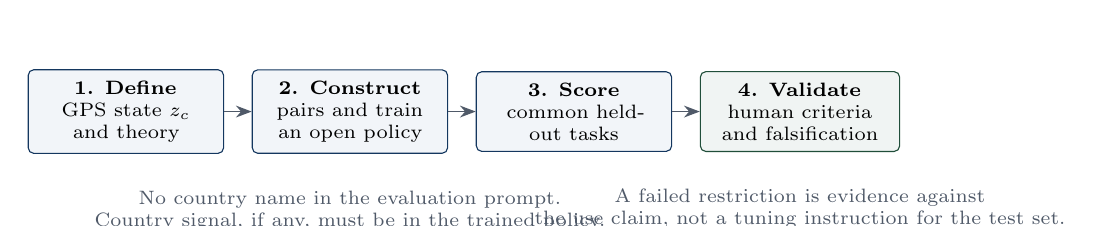
\begin{tikzpicture}[font=\scriptsize,
 box/.style={draw=econblue, rounded corners=2pt, fill=mist, align=center, text width=2.20cm, minimum height=.9cm, inner sep=4pt},
 check/.style={draw=green!75!black, rounded corners=2pt, fill=green!7, align=center, text width=2.25cm, minimum height=.9cm, inner sep=4pt},
 arr/.style={-{Stealth[length=2mm]}, line width=.65pt, color=slate}]
\node[box] (gps) {\textbf{1. Define}\\GPS state $z_c$ and theory};
\node[box, right=.35cm of gps] (train) {\textbf{2. Construct}\\pairs and train an open policy};
\node[box, right=.35cm of train] (score) {\textbf{3. Score}\\common held-out tasks};
\node[check, right=.35cm of score] (valid) {\textbf{4. Validate}\\human criteria and falsification};
\draw[arr] (gps)--(train); \draw[arr] (train)--(score); \draw[arr] (score)--(valid);
\node[font=\scriptsize\color{slate},align=center,below=.35cm of train] {No country name in the evaluation prompt.\\Country signal, if any, must be in the trained policy.};
\node[font=\scriptsize\color{slate},align=center,below=.35cm of valid] {A failed restriction is evidence against\\the use claim, not a tuning instruction for the test set.};
\end{tikzpicture}
\caption{SCA 2.0 as a specific instance of the general framework. Training is only the middle of the argument; validation determines the permitted interpretation.}
\label{fig:sca}
\end{figure}

\subsection{Identification of the moment-anchored estimator}

The training pipeline starts from a country's six-dimensional Global Preferences Survey profile $z_c$~\cite{falk2018}, which parameterizes a scenario generator $q(z_c)$ that emits preference pairs; Direct Preference Optimization adjusts an open-weight student policy so that preferred responses are more probable than rejected ones relative to a reference policy~\cite{rafailov2023}. Under the Bradley--Terry reading, the trained policy's option probabilities form a discrete-choice distribution whose implied reward margins are identified relative to the reference policy~\cite{bradley1952,rafailov2023}. Three maintained assumptions make this estimator a candidate measurement function rather than a curve fit: the aggregate moments $z_c$ are valid summaries of the population's preference-relevant attributes for the construct of interest; the scenario generator draws items exchangeably from the construct's content domain; and the Bradley--Terry model holds, so that pairwise choice probabilities are logistic in reward differences.

Under these assumptions, what is identified is the set of choice distributions consistent with the anchored moments---again a partial-identification object, in the same spirit as \eqref{eq:range}: the moments pin the anchor, but the mapping from moments to choice distributions is not unique, and the trained policy realizes one element of the identified set~\cite{manski2003}. What is not identified is cardinal utility, individual-level heterogeneity within the country, and cross-country comparability beyond the anchor scale. This is the sense in which the estimator is moment-anchored rather than item-anchored: PLURAL conditions preference training on survey item responses~\cite{plural2026}, and PALMs on language-model-synthesized construct-grounded rationales~\cite{palms2026}; both carry item-level or synthesized content into the training distribution. The present estimator anchors only on aggregate moments and inherits, in exchange, the aggregation assumption that the moments are sufficient statistics for the preference distribution---a stronger and more transparent assumption than the content assumptions of item-level pipelines, and one that the validity framework can screen: the trained adapter is a candidate measurement function $m_{\mathrm{DPO}}$ in the menu of Section~3, and its admissibility is determined by the same restrictions applied to any other measure. The screening question, not the raw policy, is the point of the paper.

\subsection{The current evidence and its proper role}
The existing pipeline has completed a useful but limited proof of concept. On 35 unseen WVS Wave 7 items, the Mexico adapter's fixed option distribution was closer to Mexican survey responses than the US adapter's on 34 items; the USA adapter degraded fit relative to the base model on both US and Mexican data. Because country labels were omitted at evaluation, these outcomes are consistent with country-specific information being represented in the adapter weights. They do not establish country-conditioned inference, calibrated response shares, or an explanation for the US degradation. Option scoring also showed under-dispersion relative to human response distributions.

These findings should motivate the benchmark; they should not carry the paper's general claim. In particular, a two-country comparison cannot demonstrate that DPO dominates persona prompting, because persona prompting and retrieval have not yet been evaluated on the same preregistered outcomes. Nor should a training-pair recovery score be treated as validity evidence, since it shares generative ancestry with the training labels. The compact evidence profile and the trust illustration are reported in Appendix~A as examples of the reporting standard, rather than as the paper's main result.

\section{What would justify the claim? A common evaluation program}
The program's decisive test is not another isolated adapter result. It is a common benchmark in which all candidate projections answer the same held-out tasks, are compared with the same human reference, and face the same negative controls. Table~\ref{tab:matrix} gives the required design.

\begin{table}[t]
\centering
\small
\caption{Minimum common evaluation matrix. A check mark means that the method must be evaluated on that surface, not that it is expected to pass.}
\label{tab:matrix}
\begin{tabularx}{\textwidth}{@{}>{\raggedright\arraybackslash}p{2.25cm} c c c c >{\raggedright\arraybackslash}X@{}}
\toprule
\textbf{Candidate} & \textbf{OOS items} & \textbf{Human criterion} & \textbf{Demographic structure} & \textbf{Placebos} & \textbf{Interpretation if it passes}\\
\midrule
Persona prompt & \checkmark & \checkmark & \checkmark & \checkmark & Reduced-form baseline\\
RAG prompt & \checkmark & \checkmark & \checkmark & \checkmark & Evidence-sensitive contextual baseline\\
DPO adapter & \checkmark & \checkmark & \checkmark & \checkmark & Candidate policy-level projection\\
Steering & \checkmark & \checkmark & \checkmark & \checkmark & Candidate controllable projection\\
Composite / PCA & \checkmark & \checkmark & \checkmark & \checkmark & Transparent non-LLM comparator\\
Experiment & --- & \checkmark & \checkmark & \checkmark & Different-method anchor\\
\bottomrule
\end{tabularx}
\end{table}

The benchmark must include at least four resolutions. First, compare country-level criterion recovery while reporting uncertainty and sensitivity to development covariates. Second, test demographic gradients within countries, where a measure must reproduce predeclared signs and magnitudes rather than merely country means. Third, compare cell means after within-country demeaning. Fourth, evaluate response distributions on items that were never used for training, prompt construction, retrieval, or measure selection. These resolutions answer different failure modes; no single correlation can replace them.

The comparator family must also be broader than LLM variants. A survey composite and PCA can outperform an elaborate agent on some outcomes; that is a substantive result, not an embarrassment. Conversely, a DPO agent that passes where a prompt fails may be useful precisely because the policy intervention produces a more stable projection. The expected outcome is a qualified frontier, not a universal ranking.

A credible superiority claim would therefore read: \emph{for a predeclared construct, population, task family, and external criteria, method $m_{\mathrm{DPO}}$ achieved better performance than persona prompting and the named alternatives, while satisfying the locked validity restrictions.} The word ``better'' must be attached to this design. It should not be used before the comparison is run.

\section{Research uses, boundaries, and release strategy}
If the benchmark supports the narrow claim above, SCA 2.0 can support several uses. It can help researchers generate hypotheses, stress-test draft questionnaires, and select between candidate instruments before fieldwork. With a construct-identified effect range, it can support power calculations across defensible effect sizes instead of relying on a single convenient prior. It may assist in piloting field or laboratory interventions by identifying questions and behavioral margins worth measuring. These uses remain subordinate to human data; the agent proposes and screens, while fieldwork adjudicates.

Three uses are not supported by the present design: polling or forecasting absolute population shares, individual-level diagnosis, and causal counterfactual claims about people. The last boundary matters. A validated agent may provide a model-based counterfactual of its own policy under a controlled intervention. That does not identify the human causal response absent an independently defensible bridge.

\subsection{Necessary extensions before a general-science submission}
A serious PNAS- or Nature-facing manuscript needs more than a polished account of two adapters. The minimum package is:
\begin{enumerate}
\item \textbf{Validate the target constructs first.} Lock construct definitions, measurement menus, thresholds, and negative controls before interpreting adapter outcomes. Expand the trust-style profile into multi-restriction networks for each GPS dimension; report empty sets where the current WVS bridge fails.
\item \textbf{Run the common benchmark.} Add persona prompting immediately and retrieval-augmented prompting where data provenance permits. Include DPO, steering, base models, survey composites, PCA, and a different-method human anchor. Pre-register the scoring and aggregation rules.
\item \textbf{Broaden the panel and its variation.} Add countries selected to span GPS profiles, linguistic settings, and baseline-model proximity; use independent survey sources where coverage allows; and reserve countries, questions, and constructs that are untouched until final evaluation.
\item \textbf{Test robustness and falsification.} Vary base models, seeds, prompt templates, item wording, calibration procedures, and training-data size. Add deliberately invalid measures, shuffled-country labels, and mismatched constructs. Report failures alongside successes.
\item \textbf{Make the artifact auditable.} Release frozen protocols, score tables where licenses permit, code, model cards, data documentation, and reproducible figures. The public claim should be reconstructible without access to private reasoning or a proprietary API.
\end{enumerate}

Open release on Hugging Face should follow, not precede, these gates. The appropriate near-term decision is \emph{release readiness}, not a premature public adapter launch: document base-model and survey licenses, remove any restricted training material, publish a model card with the permitted use claim and known failures, version the evaluation suite, and archive the exact adapter and protocol hashes. Once those conditions are met, a gated or fully public Hugging Face release is a scientific asset because it allows independent replication. Before then, an adapter download can invite stronger uses than the evidence warrants.

\section{Conclusion}
The central wager of SCA 2.0 is not that a fine-tuned language model can replace respondents. It is that social science can use AI-generated simulations more carefully than it has used generic persona prompts: by treating prompts, retrieval systems, trained policies, steering interventions, and conventional composites as competing projection functions; by testing them against a researcher-authored validity network and independent human evidence; and by reporting the set of conclusions that survives.

Culture provides a demanding first case because the relevant attributes are latent, the populations are heterogeneous, and the temptation to substitute a plausible narrative for a measurement argument is strong. SCA 2.0 combines a way to construct policy-level candidates with a way to reject them. If that combination yields a reproducible improvement over prompting, it will support a new kind of validated simulation for non-\WEIRD{} populations. If it does not, the result is still valuable: it marks the boundary of what current synthetic agents can responsibly claim.

\appendix
\section{Illustrative reporting standard: two compact evidence profiles}
This appendix records the current evidence in its proper place. It is not a substitute for the common benchmark proposed above.

\subsection{Adapter proof of concept}
Figure~\ref{fig:adapter} visualizes the present two-country result. The matched Mexico adapter beat the cross-country adapter on 34 of 35 held-out WVS questions, with mean $\Delta\mathrm{TVD}=0.1495$ and a 95\% interval $[0.0964,0.2152]$. In the US comparison, the USA adapter fit worse than both the base model and the Mexico adapter. These are distributional-alignment results for fixed outputs under unconditioned prompts, not evidence that the agent infers country at test time.

\begin{figure}[h]
\centering
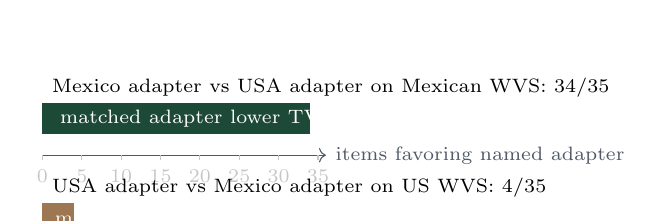
\begin{tikzpicture}[x=0.10cm,y=0.55cm,font=\scriptsize]
\draw[->,color=slate] (0,0)--(36,0) node[right]{items favoring named adapter};
\foreach \x in {0,5,...,35} \draw[gray!45] (\x,0)--(\x,-.12) node[below]{\x};
\fill[green!70!black] (0,.5) rectangle (34,1.2);
\node[anchor=west] at (0,1.55) {Mexico adapter vs USA adapter on Mexican WVS: $34/35$};
\node[anchor=west,text=white] at (1,0.85) {matched adapter lower TVD};
\fill[warm!80] (0,-1.8) rectangle (4,-1.1);
\node[anchor=west] at (0,-.75) {USA adapter vs Mexico adapter on US WVS: $4/35$};
\node[anchor=west,text=white] at (.35,-1.45) {matched};
\end{tikzpicture}
\caption{Current adapter evidence, expressed as the item-level matched-versus-cross comparison. The figure is intentionally descriptive: it does not provide a cross-method benchmark or identify a mechanism.}
\label{fig:adapter}
\end{figure}

\subsection{Why a validity layer changes the analysis}
A frozen country-level trust profile compares four WVS trust facets to GPS trust across 42 overlapping countries. At the prespecified correlation floor of $0.30$, generalized trust Q57 has $r=0.278$ and is rejected; in-group, out-group, and institutional facets have $r=0.349$, $0.303$, and $0.332$. The three-facet survivor composite has $r=0.410$. This example does not crown a universal trust measure. It shows that a familiar single item and a composite can support materially different measurement claims.

\begin{figure}[h]
\centering
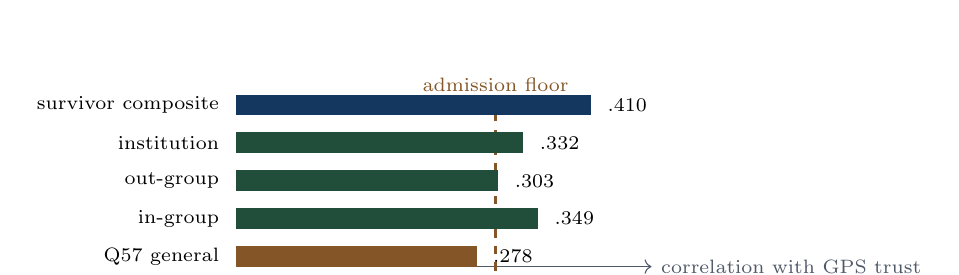
\begin{tikzpicture}[x=11cm,y=.48cm,font=\scriptsize]
\draw[->,color=slate] (0,0)--(.48,0) node[right]{correlation with GPS trust};
\draw[dashed,thick,color=warm] (.30,-.55)--(.30,4.35) node[above,text=warm]{admission floor};
\foreach \y/\lab/\val/\col in {0/{Q57 general}/.278/warm,1/{in-group}/.349/green!75!black,2/{out-group}/.303/green!75!black,3/{institution}/.332/green!75!black,4/{survivor composite}/.410/econblue} {
  \fill[\col] (0,\y) rectangle (\val,\y+.55);
  \node[anchor=east] at (-.008,\y+.27) {\lab};
  \node[anchor=west] at (\val+.008,\y+.27) {\val};}
\end{tikzpicture}
\caption{Illustrative trust validity profile. This is one convergent restriction, not a complete validation argument; the proposed program adds demographic, discriminant, known-groups, and falsification restrictions.}
\label{fig:trust}
\end{figure}

\section{Operational details of \cvp{}}
The validation engine receives a unit-by-measure score table, a researcher-authored network, a target functional, a seed, and a versioned protocol. It returns the slack for every measure-restriction pair, the admissible set, the image of the target over that set, bootstrap uncertainty over units, and a threshold grid. Run identifiers hash frozen inputs so that an output can be traced to the exact score table and protocol. The tool has no language-model calls and does not infer the researcher's theory. This separation makes it suitable both for SCA 2.0 and for non-AI measurement problems.

\section{Technical details and proofs}

\subsection{Proof of Proposition 1}
\begin{proof}[Proof sketch of Proposition~\ref{prop:consistency}]
Write $\mu(m)=\min_{r\in\mathcal{R}}s_r(m)+\delta$. Separation implies $\eta:=\min_{m\in\M}|\mu(m)|>0$. Uniform consistency \eqref{eq:uniform} gives $\Pr\bigl(\max_{m,r}|\hat{s}_r(m)-s_r(m)|<\eta/2\bigr)\to 1$; on this event $\hat{\mu}(m):=\min_r\hat{s}_r(m)+\delta$ has the sign of $\mu(m)$ for every $m$, so $\hat{\M}^*=\M^*$ with probability tending to one. On the same event the endpoints are extrema of $\hat{\beta}$ over the fixed set $\M^*$, and since $\bigl|\min_{m\in\M^*}\hat{\beta}(m)-\min_{m\in\M^*}\beta(m)\bigr|\le\max_{m\in\M}|\hat{\beta}(m)-\beta(m)|\to_p 0$ (likewise for the maximum), $[\hat L,\hat U]\to_p[L,U]$. Boundary measures, with $\mu(m)=0$, are the only obstruction: their admission is decided by sampling noise.
\end{proof}

\subsection{The coupling problem and the uncertainty band}
The plug-in range inherits two sources of sampling error: the endpoint estimates $\hat{\beta}(m)$ and the admission decision $\hat{\M}^*$. These are coupled whenever a measure's slack margin lies within estimation error of the boundary: such a measure can be admitted in one sample and rejected in the next, and if it is also a $\beta$-extreme, the endpoints move discontinuously. The reporting protocol of Section~3 addresses the coupling with three devices. First, the uncertainty band is reported per side at $\alpha/2$; under the Bonferroni reading the simultaneous event $\{L\ge \hat L_q,\ U\le \hat U_q\}$ has probability at least $1-\alpha$, but only approximately so, because the min/max functional over an estimated set is non-smooth and percentile methods for extrema can be unreliable when gaps between candidate $\beta(m)$ vanish. The band is an uncertainty summary with documented coverage properties under the stated reading, not a formal confidence region under arbitrary dependence. Second, the empty-replicate rate is reported because coverage is conditional on a non-empty admissible set; a material empty rate signals that admission itself is not robust. Third, boundary attribution makes the coupling visible: the set of measures with margin within $\kappa\cdot\mathrm{SE}$ of the boundary is reported alongside the band, and the conservative per-measure projection (Bonferroni over $|\hat{\M}^*|$) provides an outer check---if the projection is materially wider than the band, the coupling is material. In the small-$n$ regime of the application (country-level units, $n\approx 35$), per-side quantiles are coarse, and the empty rate and the boundary set are the primary honest outputs; $m$-out-of-$n$ resampling is a documented future robustness item rather than a shipped feature.

\subsection{Simultaneous coverage of the coupled band}
A complete treatment would construct a confidence region for the pair $(L,U)$---or for the random set $\M^*$ jointly with the endpoint estimates---with uniform coverage over a class of slack distributions that admit boundary measures. The natural building blocks are endpoint inference for partially identified parameters \cite{imbensmanski2004,stoye2009} applied to the intersection bounds induced by admission, together with a correction for the admission decision; the difficulty is that admission is itself a function of the sample, so the identified set is random. Sample splitting (half-sample admission, half-sample endpoints) decorrelates the two sources at the cost of effective sample size---unattractive at $n\approx 35$---and provides the cleanest benchmark for the conservativeness of the reported band. Formal results are deferred to the companion methods paper; the present paper commits to the reporting protocol of Section~3.

\subsection{Holdout pass-rate comparison}
The estimator $\hat p$ of Section~3 is a ratio of counts over the (random) survivor set. Conditional on a pre-registered holdout set and on the survivor set being non-empty with probability tending to one, its asymptotics follow from the consistency of the admissible set (Proposition~1) and a standard delta-method argument; the comparison against the baseline analogue on the same holdout set is the operational test. The formal treatment belongs with the companion methods paper.

\begin{thebibliography}{99}\small
\bibitem{aher2023} Aher, G., R. I. Arriaga, and A. T. Kalai (2023). ``Using Large Language Models to Simulate Multiple Humans and Replicate Human Subject Studies.'' \textit{ICML}.
\bibitem{argyle2023} Argyle, L. P., E. C. Busby, N. Fulda, J. R. Gubler, C. Rytting, and E. S. Wiley (2023). ``Out of One, Many: Using Language Models to Simulate Human Samples.'' \textit{Political Analysis} 31(3): 337--351.
\bibitem{borsboom2004} Borsboom, D., G. J. Mellenbergh, and J. van Heerden (2004). ``The Concept of Validity.'' \textit{Psychological Review} 111(4): 1061--1071.
\bibitem{bradley1952} Bradley, R. A., and M. E. Terry (1952). ``Rank Analysis of Incomplete Block Designs: I. The Method of Paired Comparisons.'' \textit{Biometrika} 39: 324--345.
\bibitem{campbell1959} Campbell, D. T., and D. W. Fiske (1959). ``Convergent and Discriminant Validation by the Multitrait-Multimethod Matrix.'' \textit{Psychological Bulletin} 56: 81--105.
\bibitem{capra2025} Capra, C. M., A. Gonzalez-Bonorino, and M. Pantoja (2025). ``LLMs Can Model Non-WEIRD Populations: Experiments with Synthetic Cultural Agents.'' Forthcoming, \textit{Experimental Economics}.
\bibitem{cronbach1955} Cronbach, L. J., and P. E. Meehl (1955). ``Construct Validity in Psychological Tests.'' \textit{Psychological Bulletin} 52: 281--302.
\bibitem{cvprofiles} EconLLM Lab / A. Gonzalez-Bonorino (2026). \texttt{cvprofiles}: Construct-Validity Profiles. \url{https://github.com/Bonorinoa/cvprofiles}.
\bibitem{durmus2024} Durmus, E., et al. (2024). ``Towards Measuring the Representation of Subjective Global Opinions in Language Models.'' \textit{COLM}.
\bibitem{falk2018} Falk, A., A. Becker, T. Dohmen, B. Enke, D. Huffman, and U. Sunde (2018). ``Global Evidence on Economic Preferences.'' \textit{Quarterly Journal of Economics} 133: 1645--1692.
\bibitem{henrich2010} Henrich, J., S. J. Heine, and A. Norenzayan (2010). ``The Weirdest People in the World?'' \textit{Behavioral and Brain Sciences} 33: 61--83.
\bibitem{horton2023} Horton, J. J. (2023). ``Large Language Models as Simulated Economic Agents: What Can We Learn from Homo Silicus?'' NBER Working Paper 31122.
\bibitem{ludwig2026} Ludwig, J., S. Mullainathan, and A. Rambachan (2026). ``Large Language Models: An Applied Econometric Framework.'' \textit{Annual Review of Economics} 18.
\bibitem{manski2003} Manski, C. F. (2003). \textit{Partial Identification of Probability Distributions}. Springer.
\bibitem{rafailov2023} Rafailov, R., A. Sharma, E. Mitchell, S. Ermon, C. D. Manning, and C. Finn (2023). ``Direct Preference Optimization: Your Language Model is Secretly a Reward Model.'' \textit{NeurIPS}.
\bibitem{schennach2021} Schennach, S. M. (2021). ``Measurement Systems.'' cemmap Working Paper CWP12/21.
\bibitem{dellrambachan2026} Dell, M., and A. Rambachan (2026). ``Measurement in the Age of AI: Discovery, Definition, and Observation; Construct Validity: Credibility When Measurement Is Cheap; Measurement with Validation Samples; Measurement without Random Validation Samples.'' NBER Summer Institute 2026 Methods Lecture slides, July 30.
\bibitem{bisbee2024} Bisbee, J., J. D. Clinton, C. Dorff, B. Kenkel, and J. M. Larson (2024). ``Synthetic Replacements for Human Survey Data? The Perils of Large Language Models.'' \textit{Political Analysis} 32(4): 401--416.
\bibitem{morocho2026} Taday Morocho, F., A. Cima, T. Fagni, M. Avvenuti, and S. Cresci (2026). ``Assessing the Reliability of Persona-Conditioned LLMs as Synthetic Survey Respondents.'' arXiv:2602.18462.
\bibitem{subgroupvalues2026} Tan, B. C. Z., Z. Liu, X. Yi, J. Yao, X. Xie, N. F. Chen, and R. K.-W. Lee (2026). ``Can Persona-Prompted LLMs Emulate Subgroup Values? An Empirical Analysis of Generalisability and Fairness in Cultural Alignment.'' \textit{Proceedings of ACL 2026}. arXiv:2604.12851.
\bibitem{tonneau2026} Tonneau, M., et al. (2026). ``Different Demographic Cues Yield Inconsistent Conclusions About LLM Personalization and Bias.'' arXiv:2601.18486.
\bibitem{tao2024} Tao, Y., et al. (2024). ``Cultural Bias and Cultural Alignment of Large Language Models.'' \textit{PNAS Nexus} 3(9): pgae346.
\bibitem{wangcalibration2026} Wang, Z., S. Deng, and S. Yang (2026). ``Assessing and Mitigating Miscalibration in LLM-Based Social Science Measurement.'' arXiv:2605.11954.
\bibitem{hall2026} Hall, A. B. (2026). ``AI Research Topics at PolMeth 2026.'' GitHub repository, github.com/andybhall/polmeth-2026-ai.
\bibitem{gilardi2023} Gilardi, F., M. Alizadeh, and M. Kubli (2023). ``ChatGPT Outperforms Crowd Workers for Text-Annotation Tasks.'' \textit{PNAS} 120(30): e2305016120.
\bibitem{landesvatter2026} Landesvatter, C., et al. (2026). ``Using Large Language Models for Coding Open-Ended Survey Responses.'' \textit{Survey Research Methods} (in press). arXiv:2506.14634.
\bibitem{glaeser2000} Glaeser, E. L., D. I. Laibson, J. A. Scheinkman, and C. L. Soutter (2000). ``Measuring Trust.'' \textit{Quarterly Journal of Economics} 115(3): 811--846.
\bibitem{sapienza2013} Sapienza, P., A. Toldr\'a-Simats, and L. Zingales (2013). ``Understanding Trust.'' \textit{Economic Journal} 123(573): 1313--1332.
\bibitem{butler2016} Butler, J. V., P. Giuliano, and L. Guiso (2016). ``The Right Amount of Trust.'' \textit{Journal of the European Economic Association} 14(5): 1155--1188.
\bibitem{falk2023} Falk, A., A. Becker, T. Dohmen, D. Huffman, and U. Sunde (2023). ``The Preference Survey Module: A Validated Instrument for Measuring Risk, Time, and Social Preferences.'' \textit{Management Science} 69(4): 1935--1950.
\bibitem{hu2008} Hu, Y., and S. M. Schennach (2008). ``Instrumental Variable Treatment of Nonclassical Measurement Error Models.'' \textit{Econometrica} 76(1): 195--216.
\bibitem{chen2011} Chen, X., H. Hong, and D. Nekipelov (2011). ``Nonlinear Models of Measurement Errors.'' \textit{Journal of Economic Literature} 49(4): 901--937.
\bibitem{ziems2024} Ziems, C., et al. (2024). ``Can Large Language Models Transform Computational Social Science?'' \textit{Computational Linguistics} 50(1): 237--291.
\bibitem{park2024} Park, J. S., C. J. O'Brien, C. J. Cai, M. R. Morris, P. Liang, and M. S. Bernstein (2024). ``Generative Agent Simulations of 1,000 People.'' arXiv:2411.10109.
\bibitem{manning2024} Manning, B. S., K. Zhu, and J. J. Horton (2024). ``Automated Social Science: Language Models as Scientist and Subjects.'' NBER Working Paper 32381. arXiv:2404.11794.
\bibitem{plural2026} Agarwal, D., A. Shukla, T. Goyal, and A. Vashistha (2026). ``PLURAL: A Global Dataset for Value Alignment.'' arXiv:2607.08034.
\bibitem{palms2026} Dey, P., B. Joshi, P. Poddar, J. Zhao, and E. Ferrara (2026). ``PALMs: Using Multi Construct-Grounded Rationales for Modeling Population Preferences in LLMs.'' arXiv:2608.01458.
\bibitem{licht2025} Licht, H., R. Sarkar, P. Y. Wu, P. Goel, N. Stoehr, E. Ash, and A. M. Hoyle (2025). ``Measuring Scalar Constructs in Social Science with LLMs.'' \textit{EMNLP 2025}. arXiv:2509.03116.
\bibitem{bean2025} Bean, K., et al. (2025). ``Measuring What Matters: Construct Validity in LLM Benchmarks.'' arXiv:2511.04703.
\bibitem{freiesleben2026} Freiesleben, T. (2026). ``LLM Capability Benchmarks Require Nomological Networks.'' PhilSci-Archive 29807. % TODO: verify exact title
\bibitem{coston2026} Coston, A. (2026). ``Falsifying Discriminant Validity of Predictive Algorithms.'' \textit{FAccT 2026}. arXiv:2601.17146.
\bibitem{messick1995} Messick, S. (1995). ``Validity of Psychological Assessment: Validation of Inferences from Persons' Responses and Performances as Scientific Inquiry into Score Meaning.'' \textit{American Psychologist} 50(9): 741--749.
\bibitem{kane2013} Kane, M. T. (2013). ``Validating the Interpretations and Uses of Test Scores.'' \textit{Journal of Educational Measurement} 50(1): 1--73.
\bibitem{ogutyin2026} Ogut, B., and M. Yin (2026). ``Partial Identification with Multiple Nonlinear Measurements of a Latent Regressor.'' arXiv:2607.12219.
\bibitem{chenrambachantamer2026} Chen, X., A. Rambachan, and E. Tamer (2026). ``Partial Identification from LLM Prompts.'' arXiv:2606.15031.
\bibitem{molinari2020} Molinari, F. (2020). ``Microeconometrics with Partial Identification.'' In \textit{Handbook of Econometrics}, Vol. 7A, 355--486. Elsevier.
\bibitem{proxy2026} Li, B., T. Yu, K. J. L. Koa, and K.-W. Huang (2026). ``The Proxy Presumption: From Semantic Embeddings to Valid Social Measures.'' \textit{Proceedings of ACL 2026}. arXiv:2605.07409.
\bibitem{desai2026} Desai, M., D. Card, and A. Z. Jacobs (2026). ``Validating LLMs in Social Science: Epistemic Threats and Emerging Norms.'' arXiv:2607.07915.
\bibitem{disca2026} Kiet, H. T., D. S. D. Minh, T. Nguyen, C.-N. Tran, P.-H. Pham, N. L. P. Quy, A. Han, and L. Tran-Thanh (2026). ``Training-Free Cultural Alignment of Large Language Models via Persona Disagreement.'' arXiv:2605.10843.
\bibitem{halterman2024} Halterman, A., and K. A. Keith (2024). ``Codebook LLMs: Evaluating LLMs as Measurement Tools for Political Science Concepts.'' \textit{Political Analysis}. arXiv:2407.10747.
\bibitem{imbensmanski2004} Imbens, G. W., and C. F. Manski (2004). ``Confidence Intervals for Partially Identified Parameters.'' \textit{Econometrica} 72(6): 1845--1857.
\bibitem{stoye2009} Stoye, J. (2009). ``More on Confidence Intervals for Partially Identified Parameters.'' \textit{Econometrica} 77(4): 1299--1315.
\end{thebibliography}
\end{document}
